\section{Typed realizability}
\label{sec:typed-realizability}

RZ is based on \emph{typed realizability} by John
Longley~\cite{Longley99}. It is the variant of realizability that most
directly corresponds to the informal view that programmers have in
mind when thinking about an implementation of a structure.

We motivate and explain typed realizability and its relationship with
real-world programming by way of example. Suppose we are asked to
design a data structure for the set $\mathcal{G}$ of all finite
simple\footnote{At most one arrow between any two vertices.}
directed graphs with vertices labeled by distinct integers. An exemplar
directed graph~$G$ is shown in Figure~\ref{fig:digraph}.
%
\begin{figure}
  \centering
  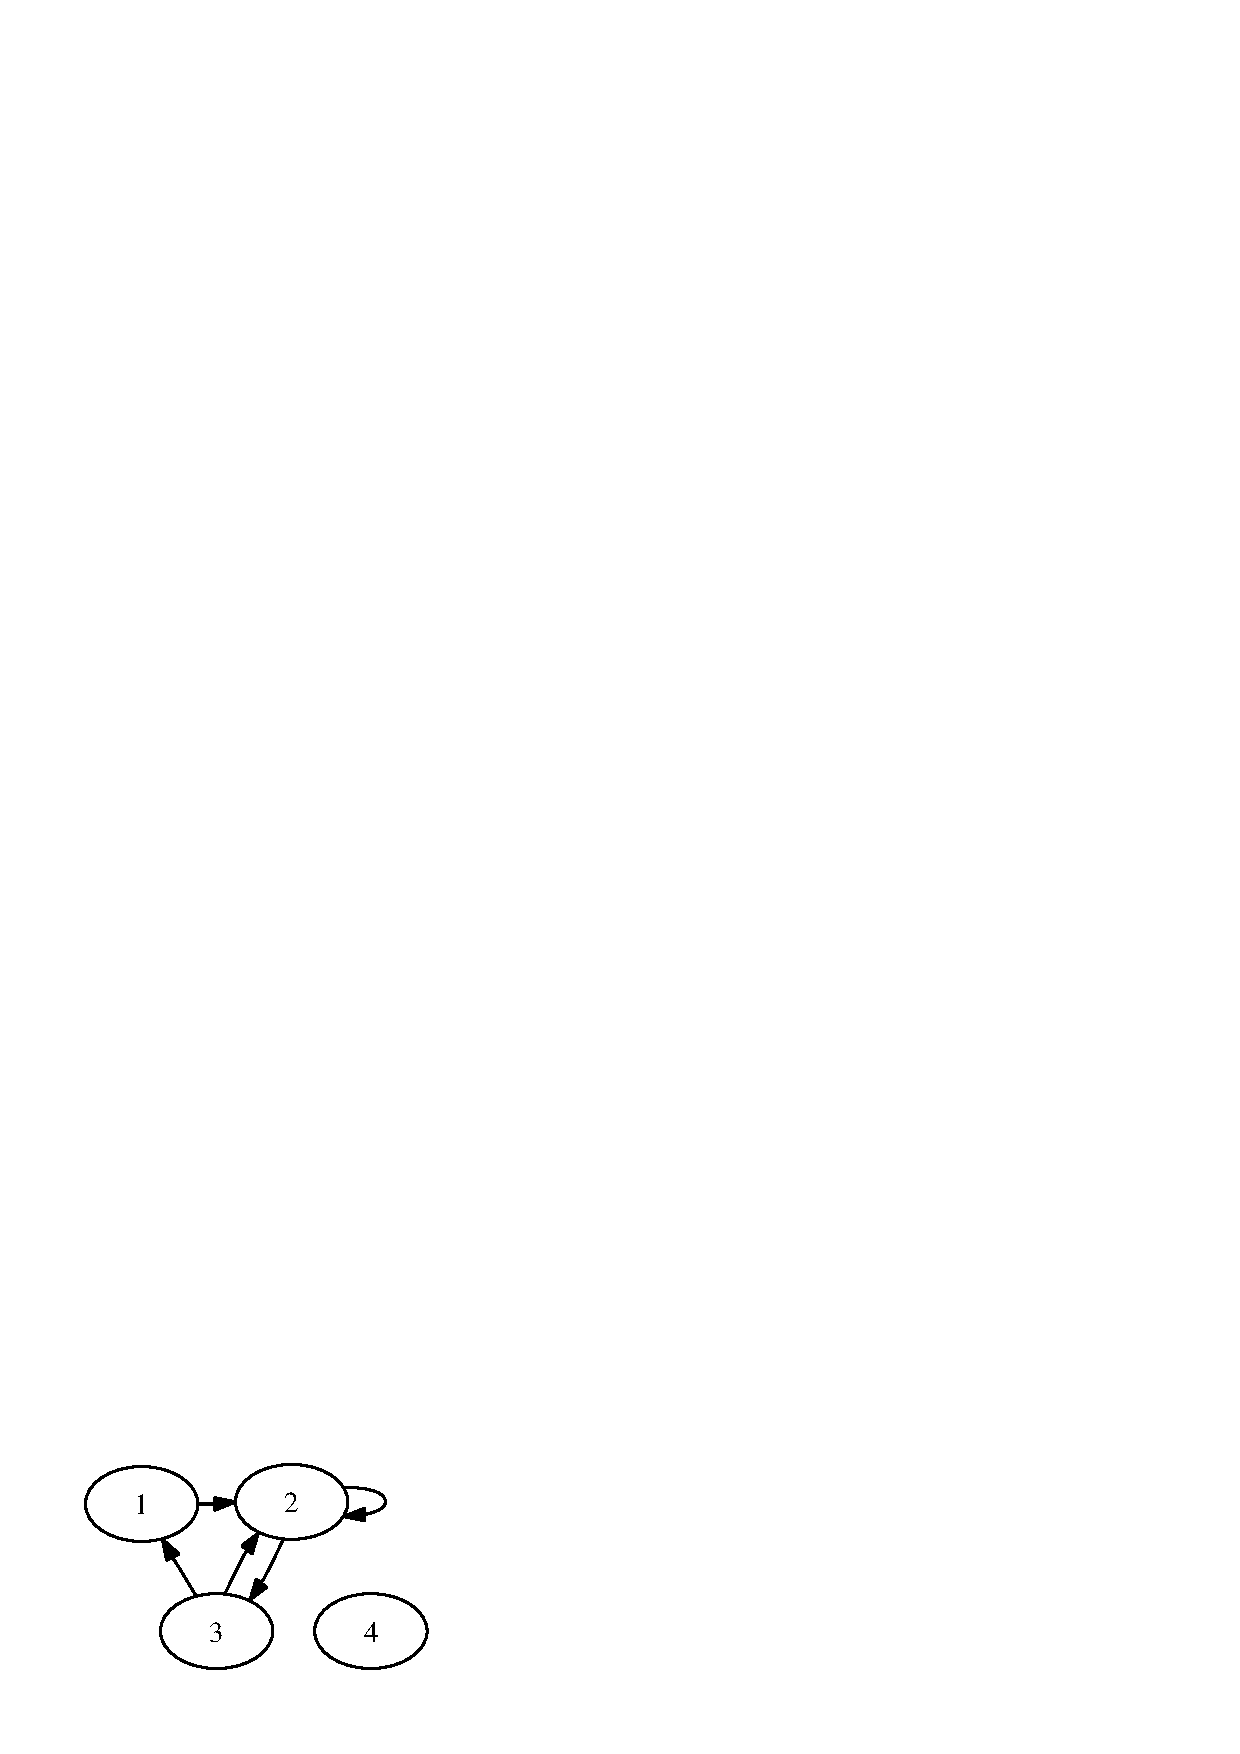
\includegraphics[width=0.4\textwidth]{digraph}
  \caption{A finite directed graph $G$}
  \label{fig:digraph}
\end{figure}
%
A common representation is a pair of lists $(\ell_V, \ell_A)$, where
$\ell_V$ is the list of vertex labels and $\ell_A$ is the \emph{adjacency list} 
representing the arrows by pairing the labels of each source and target.
In our example, $\ell_V = [1; 2;
3; 4]$ and $\ell_A = [(1,2); (2,2); (2,3); (3,2); (3;1)]$. Thus we
define the datatype of graphs to be\footnote{We use Ocaml notation in
  which $\clist{t}$ classifies finite lists of elements of type~$t$, and
  $t_1 * t_2$ classifies pairs containing a value of type $t_1$ and and 
  value of type $t_2$.}
%
\begin{equation*}
  \ctype \mathtt{graph} = \clist{\cint} * \clist{(\cint * \cint)}
\end{equation*}
%
However, this is not a complete description of the representation, as
there are invariants and conditions which are not expressed directly
in the programming language, such as:
%
\begin{enumerate}
\item The order in which vertices and arrows are listed is not
  important, e.g., $[1;2;3;4]$ and $[4;1;2;3]$ represent the same vertices.
\item Each vertex and arrow must be listed exactly once.
\item The source and target of each arrow must appear in the list of vertices.
\end{enumerate}
%
An implementation of the mathematical set~$\mathcal{G}$ must thus tell
us not only what the underlying datatype $\mathtt{graph}$ is, but also
which values of type $\mathtt{graph}$ represent which elements
of~$\mathcal{G}$. As we shall see next, all of this can be expressed
either as a \emph{realizability relation} or a \emph{partial
  equivalence relation (per)}.


\subsection{Modest sets and pers}
\label{sec:modest-sets-pers}

We now give the formal definition of typed realizability, as it
applies to OCaml. Other general-purpose programming languages could be
used instead, as long as they provide the usual ground types, product
and function types.\footnote{ It is also convenient to work with a
language that supports sum types, as this allows a more natural
representation of disjoint unions.}

Let $\Type$ be the collection of all (non-parametric) OCaml types. To
each type $t \in \Type$ we assign the set $\values{t}$ of values of
type~$t$ which behave \emph{functionally} in the sense
of~\cite{longley99when}. Such values are represented by terminating
expressions which do not raise exceptions or return different results
on different invocations, although they \emph{may} use exceptions,
store, and other computational effects, provided they behave as if
they did not. A useful example of a functional value using store is
presented in Section~\ref{sec:we-show-modulus-of-continuity-example}.
Note also that a functional value of a functional type may diverge as
soon as it is applied, e.g., if we define
$\cletrec{f\;(x:\cint):\cint}{f\;x}$ then $f \in \values{\cint \to
  \cint}$. The collection $\Type$ with the assignment of functional
values $|t|$ to each $t \in \Type$ forms a \emph{typed partial
  combinatory algebra (TPCA)}, which provides a theoretical basis for
the definition of a realizability model that suits our needs.

Going back to our example, we see that to implement the set of
directed graphs $\mathcal{G}$ is to specify a datatype
$\typeOf{\mathcal{G}} = \mathtt{graph}$ together with a
\emph{realizability relation} $\rz_{\mathcal{G}}$ between
$\mathcal{G}$ and $\values{\mathtt{graph}}$. The meaning of $(\ell_V,
\ell_A) \rz_\mathcal{G} G$ is ``OCaml value $(\ell_V, \ell_A)$ represents
(realizes, implements) graph $G$''. There are two natural conditions
that $\rz_\mathcal{G}$ ought to satisfy: (1) for every $G \in
\mathcal{G}$ there should be at least one realizer $(\ell_V, \ell_A)$
representing it, and (2) if $(\ell_V, \ell_A)$ represents both $G$ and
$G'$ then $G = G'$. The latter condition is called \emph{modesty} and
is not strictly necessary for the development of the theory, though it
is something that programmers would naturally expect to hold. If
$(\ell_V, \ell_A)$ and $(\ell'_V, \ell'_A)$ represent the same graph,
we say that they are \emph{equivalent} and write $(\ell_V, \ell_A)
\per_\mathcal{G} (\ell'_V, \ell'_A)$. The relation $\per_\mathcal{G}$
is a \emph{partial} equivalence relation (symmetric and transitive,
but not reflexive) because not every $(\ell_V, \ell_A) \in
\values{\mathtt{graph}}$ represents a graph.

\bigskip

A general definition is in order. A \emph{modest set} is a triple $A =
(\setOf{A}, \typeOf{A}, {\rz_A})$ where $\setOf{A}$ is the
\emph{underlying set}, $\typeOf{A} \in \Type$ is the \emph{underlying
  type}, and $\rz_A$ is a \emph{realizability relation} between
$\values{\typeOf{A}}$ and $\setOf{A}$, satisfying
% 
\begin{enumerate}
\item \emph{totality:} for every $x \in \setOf{A}$ there is $v \in
  \typeOf{A}$ such that $v \rz_A x$, and
\item \emph{modesty:} if $u \rz_A x$ and $u \rz_A y$ then $x = y$.
\end{enumerate}
%
The \emph{support} of $A$ is the set $\support{A} = \set{v \in
  \typeOf{A} \such \xsome{x}{\setOf{A}}{v \rz_A x}}$ of those values
which realize something. We define the relation $\per_A$ on
$\values{\typeOf{A}}$ by
%
\begin{equation*}
  u \per_A v
  \iff
  \some{x}{\setOf{A}}{u \rz_A x \land v \rz_A x} \;.
\end{equation*}
%
From totality and modesty of $\rz_A$ it follows that $\rz_A$ is a per,
i.e., symmetric and transitive. Observe that $\support{A} = \set{v \in
  \values{\typeOf{A}} \such v \per_A v}$, whence $\per_A$
restricted to $\support{A}$ is an equivalence relation. In fact, we
may recover a modest set up to isomorphism from $\typeOf{A}$ and
$\per_A$ by taking $\setOf{A}$ to be the set of equivalence classes of
$\per_A$, and $v \rz_A x$ to mean $v \in x$.

The two views of implementations, as modest sets $(\setOf{A},
\typeOf{A}, {\rz_A})$, and as pers $(\typeOf{A}, {\per_A})$, are
equivalent. In RZ we use pers because they refer only to types and
values, as opposed to arbitrary sets. Nevertheless, it is useful to
understand how modest sets and pers arise from natural considerations
about programming practice.

Modest sets form a category whose objects are modest sets and
morphisms are the realized functions. A \emph{realized function} $f :
A \to B$ is a function $f : \setOf{A} \to \setOf{B}$ for which that there
exists $v \in \values{\typeOf{A} \to \typeOf{B}}$ such that, for all
$x \in \setOf{A}$ and $u \in \typeOf{A}$,
%
\begin{equation}
  \label{eq:rz-function-space}
  u \rz_A x \implies v\;u \rz_B f(x) \;.
\end{equation}
%
This condition is just a mathematical expression of the usual idea
that~$v$ is an implementation of~$f$, since~$v$ does to realizers
what~$f$ does to the elements they represent.

The equivalent category of pers has as objects pairs $A = (\typeOf{A},
{\per_A})$ where $\typeOf{A} \in \Type$ and $\per_A$ is a per on
$\values{\typeOf{A}}$. A morphism $A \to B$ is represented by $v
\in \values{\typeOf{A} \to \typeOf{B}}$ such that, for all $u, u'
\in \support{A}$,
%
\begin{equation}
  \label{eq:per-exponential}
  u \per_A u' \implies v\;u \per_B v\;u' \;.
\end{equation}
%
Values $v$ and $v'$ which both satisfy~\eqref{eq:per-exponential}
represent the same morphism if, for all $u, u' \in \support{A}$,
%
\begin{equation*}
  u \per_A u' \implies v\;u \per_B v'\;u' \;.
\end{equation*}

The category of modest sets has a very rich structure. For example, we
may form a cartesian product $A \times B$ of modest sets $A$ and $B$
by
%
\begin{align*}
  \setOf{A \times B} &= \setOf{A} \times \setOf{B},\\
  \typeOf{A \times B} &= \typeOf{A} * \typeOf{B},\\
  p \rz_{A \times B} (x,y) &\iff
  \cfst{p} \rz_A x \land \csnd{p} \rz_B y.
\end{align*}
%
The projections $\pi_1 : A \times B \to A$ and $\pi_2 : A \times B \to
B$ are realized by $\mathtt{fst}$ and $\mathtt{snd}$, respectively.

The morphisms between modest sets~$A$ and~$B$ again form a modest set
$B^A$, also written as $A \to B$, called the \emph{exponential} of~$A$
and~$B$, with the underlying set
%
\begin{equation*}
  \setOf{B^A} =
  \set{f : \setOf{A} \to \setOf{B} \such \text{$f$ is a realized function}},
\end{equation*}
%
the underlying type
%
\begin{equation*}
  \typeOf{B^A} = \typeOf{A} \to \typeOf{B},
\end{equation*}
%
and the realizability relation $\rz_{B^A}$ defined
by~\eqref{eq:rz-function-space}. The evaluation map $e : B^A \times A
\to B$, $e(f,x) = f(x)$ is realized by Ocaml application,
$\cfun{(u,v)}{u\;v}$. If a function $f : C \times A \to B$ is realized
by $v$, then its transpose $\tilde{f} : C \to B^A$, $\tilde{f}(z)(x) =
f(z,x)$, is realized by $\cfun{z\;x}{v \; (z,x)}$. This shows that the
category of modest sets is cartesian closed. In
Section~\ref{sec:realizability-interpretation} we review other
canonical constructions on modest sets.

\bigskip

As an example we consider the cyclic group on seven elements $(\ZZ_7,
0, {-}, {+})$. To implement the group, we must give a representation
of $\ZZ_7$ as a modest set~$Z = (\ZZ_7, \typeOf{Z}, {\rz_Z})$, and
provide realizers for the neutral element~$0$, negation~$-$, and
addition~$+$. We represent the elements of~$\ZZ_7 = \set{0, 1, \ldots,
  6}$ with values of type $\typeOf{Z} = \cint$. We allow any integer
$v \in \values{\cint}$ to represent the element $v
\mathbin{\mathrm{mod}} 7$,
%
\begin{equation*}
  v \rz_Z k \iff v \mathbin{\mathrm{mod}} 7 = k \;.
\end{equation*}
%
The neutral elements $0$ is represented by~$0$, while negation and
addition are implemented by
%
\begin{align*}
  &\clet{\mathtt{neg}\; k}{-(k \cmod 7)} \\
  &\clet{\mathtt{add}\; (k, m)}{(k \cmod 7) + (m \cmod 7)}
\end{align*}
%
The expected $\clet{\mathtt{neg}\; k}{-k}$ and $\clet{\mathtt{add}\;
  k\; m}{k+m}$ do not work because of overflow at values that exceed
$2^{30}$ (in Ocaml on a 32-bit machine). We could avoid the overflow
worries by taking an isomorphic representation in which the only valid
realizers are $0$, $1$, \ldots, $6$, and negation and addition
realized by $\clet{\mathtt{neg}\; k}{7 - k}$ and $\clet{\mathtt{add}\;
  k\; m}{(k + m) \cmod 7}$, respectively.

The modest set~$Z$ also has \emph{decidable equality}, which means
that the characteristic map $\mathrm{eq} : Z \times Z \to
\set{\mathtt{false}, \mathtt{true}}$ of equality is realized, namely
by\footnote{Incidentally, $\cfun{(k,m)}{(k - m) \cmod 7 = 0}$ does not
  decide equality because of possible overflow in subtraction, whereas
  $\cfun{(k,m)}{k \cmod 7 = m \cmod 7}$ does not work because in Ocaml
  $a \cmod b$ is negative when~$a$ is negative, e.g., $(-10) \cmod 7 =
  -3$ instead of the expected $4$.} $\cfun{(k,m)}{(k \cmod 7 - m \cmod
  7) \cmod 7 = 0}$. However, not all modest sets have decidable
equality, since there may not be a decision procedure for determining
whether two realizers represent the same element. In particular, this
would happen if we implemented a semigroup with an undecidable word
problem~\cite{post47:_recur_unsol_probl_thue}.


\subsection{Interpretation of logic}
\label{sec:interpretation-logic}

In the realizability interpretation of logic, each formula~$\phi$ is
assigned a set of \emph{realizers} which can be thought of as
computations that witness the validity of~$\phi$. The situation is
somewhat similar (but not equivalent) to the propositions-as-types
translation of logic into type theory, where the proofs of a
proposition correspond to terms of the corresponding type. More
precisely, to each formula~$\phi$ we assign an underlying type
$\typeOf{\phi}$ of realizers. However, unlike in the
propositions-as-types translation, not all terms of type
$\typeOf{\phi}$ are necessarily valid realizers for~$\phi$, and some
terms which are realizers may not correspond to any proofs, for
example, if they denote partial functions or use computational
effects.

We write $t \rz \phi$ when $t \in \values{\typeOf{\phi}}$ is a
realizer for~$\phi$. The underlying types and the realizability
relation~$\rz$ are defined inductively on the structure of~$\phi$; an
outline is shown in Figure~\ref{fig:rz-logic}. We say that a
formula~$\phi$ is \emph{valid} if it has at least one realizer.
%
\begin{figure*}
  \textbf{Underlying types of realizers:}
  \begin{xalignat*}{2}
    \typeOf{\itrue} &= \mathtt{unit} &
    \typeOf{\ifalse} &= \mathtt{unit} \\
    \typeOf{\iequal{x}{y}} &= \mathtt{unit} &
    \typeOf{\iand{\phi}{\psi}} &= \oprod{\typeOf{\phi}}{\typeOf{\psi}} \\
    \typeOf{\iimply{\phi}{\psi}} &= \oarrow{\typeOf{\phi}}{\typeOf{\psi}} &
    \typeOf{\ior{\phi}{\psi}} &=
    \osumtyx{\mathtt{or}_1}{\typeOf{\phi_1}}{\mathtt{or}_2}{\typeOf{\phi_2}} \\
    \typeOf{\iforall{x}{A}{\phi}} &= \oarrow{\typeOf{A}}{\typeOf{\phi}} &
    \typeOf{\iexists{x}{A}{\phi}} &= \oprod{\typeOf{A}}{\typeOf{\phi}}
  \end{xalignat*}
  \textbf{Realizers:}
  \begin{align*}
    () \rz \itrue & \\
    () \rz \iequal{x}{y}
    &\quad\text{iff}\quad 
    x = y
    \\
    (t_1,t_2) \rz \iand{\phi}{\psi}
    &\quad\text{iff}\quad
    \text{$t_1 \rz \phi$ and $t_2 \rz \psi$}
    \\
    t \rz \iimply{\phi}{\psi}
    &\quad\text{iff}\quad
    \text{for all $u \in \typeOf{\phi}$, if $u \rz \phi$ then $t\,u
      \rz \psi$}
    \\
    \oinj{\mathtt{or}_1}{t} \rz \ior{\phi}{\psi}
    &\quad\text{iff}\quad
    \text{$t \rz \phi$}
    \\
    \oinj{\mathtt{or}_2}{t} \rz \ior{\phi}{\psi}
    &\quad\text{iff}\quad
    \text{$t \rz \psi$}
    \\
    t \rz \iforall{x}{A}{\phi(x)}
    &\quad\text{iff}\quad
    \text{for all $u \in \typeOf{A}$, if $u \rz_A x$ then $t\,u \rz \phi(x)$}
    \\
    (t_1, t_2) \rz \iexists{x}{A}{\phi(x)}
    &\quad\text{iff}\quad
    \text{$t_1 \rz_A x$ and $t_2 \rz \phi(x)$}
  \end{align*}
  \caption{Realizability interpretation of logic (outline)}
  \label{fig:rz-logic}
\end{figure*}

We illustrate how the realizability interpretation extracts the
computational content of a proposition. To make an interesting
example, suppose we already implemented the structure of real
numbers~$\RR$ as a modest set~$R = (\RR, \mathtt{real}, {\rz_R})$, and
consider the statement that every cubic $x^3 + a x + b$ has a root,
%
\begin{equation}
  \label{eq:square-root}%
  \iforall{a}{R}{\iforall{b}{R}{\iexists{x}{R}{\iequal{x^3 + a x + b}{0}}}}.
\end{equation}
%
By computing according to Figure~\ref{fig:rz-logic}, we find out that
a realizer is a value~$r$ of type
$\oarrow{\mathtt{real}}{\oarrow{\mathtt{real}}{\oprod{\mathtt{real}}{\mathtt{unit}}}}$
such that, whenever $t$ realizes $a \in \RR$ and $u$ realizes $b \in
\RR$, then $\oapp{\oapp{r}{t}}{u} = (v, w)$ with $v$ realizing a real
number~$x$ such that $x^3 + a x + b = 0$, and $w$ is irrelevant. This
can be ``optimized'' to a realizer of type
$\oarrow{\mathtt{real}}{\oarrow{\mathtt{real}}{\mathtt{real}}}$ which
does not bother to compute the irrelevant second component. In essence
then, a realizer~$r$ for~\eqref{eq:square-root} computes a root of the
cubic equation. Note that $r$ is \emph{not} extensional, i.e.,
different realizers~$t$ and~$u$ for the same~$a$ and~$b$ may result in
different roots of the cubic. To put this in another way, $r$ realizes
a \emph{multi-valued} function\footnote{The multi-valued nature of the
  realizer comes from the fact that it computes \emph{any one} of many
  values, not that it computes \emph{all} of the many values.} rather
than a modest set morphism. It is well known in computable mathematics
that certain operations, such as equation solving, must necessarily be
multi-valued in order to be computable as well. They arise naturally
in RZ as translations of $\forall\exists$~statements.

There are propositions whose realizers are ``irrelevant'' or free of
computational content. For example, realizers for $\itrue$ and
equality have type $\ounit$. Another example is a negation
$\inot{\phi}$, which is defined to be the same as
$\iimply{\phi}{\ifalse}$, whose realizers have type
$\oarrow{\typeOf{\phi}}{\ounit}$. Sometimes only a part of a realizer
is computationally irrelevant, as we saw in the last example.
Propositions which are free of any computational content are
characterized as the \emph{$\lnot\lnot$-stable propositions}. A
proposition~$\phi$ is said to be $\lnot\lnot$-stable, or just
\emph{stable} for short, when $\iimply{\inot{\inot{\phi}}}{\phi}$ is
valid. Any \emph{negative} proposition, i.e., one built from $\itrue$,
$\ifalse$, $=$, $\land$, $\Rightarrow$ and $\forall$ is stable, but
there may be other propositions which are stable and are not written
in the negative form.

It would be unproductive to bother a programmer with requirements for
useless code, so RZ has a \emph{thinning} phase, see
Section~\ref{sec:translation}, which optimizes away specifications for
computationally irrelevant realizers.

\subsection{Uniform families of modest sets}
\label{sec:uniform-families}

Many structures are naturally viewed as families of sets, or sets
depending on parameters, or \emph{dependent types} as they are called
in type theory. For example, the $n$-dimensional Euclidean space
$\RR^n$ depends on the dimension $n \in \NN$, the Banach space
$\mathcal{C}([a,b])$ of uniformly continuous real functions on the
closed interval $[a,b]$ depends on $a, b \in \RR$ such that $a < b$,
etc. In general, a family of sets $\family{A_i}{i \in I}$ is an
assignment of a set $A_i$ to each $i \in I$ from an \emph{index
  set}~$I$.

In the category of modest sets the appropriate notion is that of a
\emph{uniform} family~$\family{A_i}{i \in I}$, which is an assignment
of a modest set $A_i = (\setOf{A_i}, \typeOf{A}, {\rz_{A_i}})$ to each
$i \in \setOf{I}$, where $I$ is an index modest set,
cf.~\cite{Jacobs,Birkedal}. The uniformity comes from the requirement
that all the~$A_i$'s share the same underlying type~$\typeOf{A_i} =
\typeOf{A}$. It is a desirable restriction from the implementation
point of view, because it removes dependencies at the level of types.
Note also that there is no dependency on the realizers, only on the
elements of the underlying set.

A morphism $f : \family{A_i}{i \in I} \to \family{B_i}{i \in I}$ is a
family $\family{f_i : \setOf{A_i} \to \setOf{B_i}}{i \in I}$ of
uniformly realized maps, which means that there exists $u \in
\values{\typeOf{I} \to \typeOf{A} \to \typeOf{B}}$ such that,
%
\begin{equation*}
  v \rz_I i \land w \rz_{A_i} x \implies u\; v \; w \rz_{B_i} f_i(x)
\end{equation*}
%
for all $i \in I$, $v \in \values{\typeOf{I}}$, $x \in \setOf{A_i}$,
and $w \in \values{\typeOf{A}}$.

We may form the \emph{sum} $\depsum{i \in I}{A_i}$ of a uniform family
$\family{A_i}{i \in I}$ as
%
\begin{align*}
  \setOf{\depsum{i \in I}{A_i}} &=
  \set{\pair{i,x} \such i \in \setOf{I} \land x \in \setOf{A_i}}
  \\
  \typeOf{\depsum{i \in I}{A_i}} &=
  \typeOf{I} \times \typeOf{A}
  \\
  (u,v) \rz_{\depsum{i \in I}{A_i}} (i,x)
  &\iff
  u \rz_I i \land v \rz_{A_i} x
\end{align*}
%
and the \emph{product} $\depprod{i \in I}{A_i}$ as
%
\begin{align*}
  \setOf{\depprod{i \in I}{A_i}} &=
  \set{f : \setOf{I} \to {\textstyle \bigcup_{i \in \setOf{I}} \setOf{A_i}} \such
    \xall{i}{\setOf{i}}{f(i) \in \setOf{A_i}}}
  \\
  \typeOf{\depprod{i \in I}{A_i}} &=
  \typeOf{I} \to \typeOf{A}
  \\
  u \rz_{\depprod{i \in I}{A_i}} f
  &\iff
  \xall{i}{I}{\all{v}{\typeOf{I}}{
      v \rz_I i \implies
      u \; v \rz_{A_i} f(i)
    }}.
\end{align*}
%
These constructions allow us to interpret (extensional) dependent type
theory in the category of modest sets.

As an example of a uniform family we consider the cyclic group
$(\ZZ_n, 0, {-}, {+})$ of order~$n$. To keep things simple, we assume
that~$n$ ranges over natural numbers that can be represented by
type~$\cint$. More precisely, let $N$ be the modest set
%
\begin{align*}
  & \setOf{N} = \set{1, \ldots, 2^{30}} \\
  & \typeOf{N} = \cint \\
  & v \rz_N n \iff v = n.
\end{align*}
%
The uniform family $\family{Z_n}{n \in N}$ is like the above example
of the cyclic group of order~$7$, with $7$ replaced by~$n$:
%
\begin{align*}
  & \setOf{Z_n} = \ZZ_n = \set{0, 1, \ldots, n - 1}
  \\
  & \typeOf{Z_n} = \cint
  \\
  & v \rz_{Z_n} k \iff v \mathbin{\mathrm{mod}} n = k
  \\
  & \clet{\mathtt{neg} \; n \; k }{- (k \cmod n)}
  \\
  & \clet{\mathtt{add} \; n \; (k,m)}{k \cmod n + m \cmod n}.
\end{align*}
%
Another change is the additional parameter~$n$ accepted by the
realizers for negation and addition. The definitions make sense for
any $n \in \setOf{N}$, but for too large a value overflow might occur.
If we expect the implementation to be used with such values, it is
more prudent to replace the type~$\cint$ with an implementation of
arbitrary size integers.

\internal{Andrej}{I will polish this up when I see how the rest goes.}

%%% Local Variables: 
%%% mode: latex
%%% TeX-master: "cie"
%%% End: 
